
\subsection{The partial differential operator}

\subsubsection{Differential}

When we change the value of an input to a function, we also change the output. We can examine these changes.

Consider the value of a function \(f(x)\) at points \(x_1\) and \(x_2\).

\(y_1=f(x_1)\)

\(y_2=f(x_2)\)

\(y_2-y_1=f(x_2)-f(x_1)\)

\(\dfrac{y_2-y_1}{x_2-x_1}=\dfrac{f(x_2)-f(x_1)}{x_2-x_1}\)

Let's define \(x_2\) in terms of its distance from \(x_1\):

\(x_2=x_1+\epsilon\)

\(\dfrac{y_2-y_1}{\epsilon }=\dfrac{f(x_1+\epsilon )-f(x_1)}{\epsilon }\)

We define the differential of a function as:

\(\dfrac{\delta y}{\delta x}=\lim_{\epsilon \rightarrow 0^+}\dfrac{f(x+\epsilon )-f(x)}{\epsilon }\)

If this is defined, then we say the function is differentiable at that point.

\subsubsection{Differential operator}

\subsubsection{Graph test}


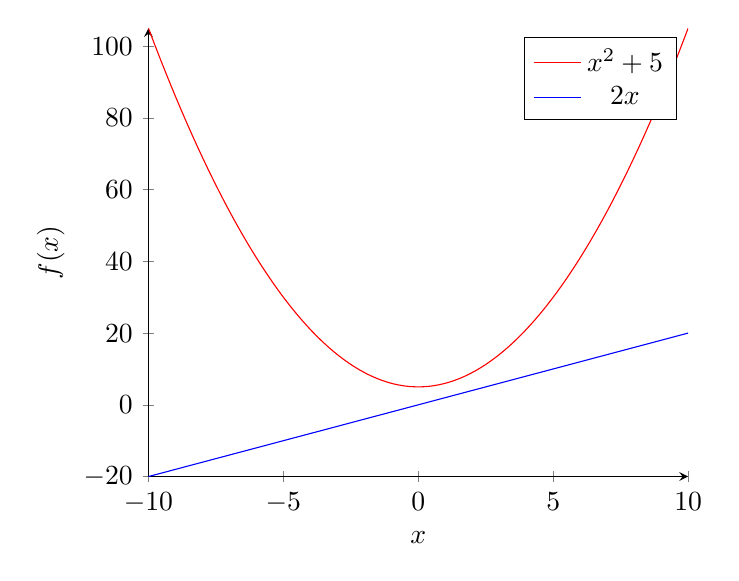
\begin{tikzpicture}
\begin{axis}[
    axis lines = left,
    xlabel = $x$,
    ylabel = {$f(x)$},
]
%Below the red parabola is defined
\addplot [
    domain=-10:10, 
    samples=100, 
    color=red,
]
{x^2 + 5};
\addlegendentry{$x^2 + 5$}
%Here the blue parabloa is defined
\addplot [
    domain=-10:10, 
    samples=100, 
    color=blue,
    ]
{2 * x};
\addlegendentry{$2x$}
 
\end{axis}
\end{tikzpicture}


